%!Mode:: "TeX:UTF-8"
\begin{frame}
    \begin{center}
        \LARGE \tt{TRANSFER SYSTEM DESIGN}
    \end{center}
\end{frame}

\begin{frame}
    \frametitle{Introduction to the Transfer System}
    \begin{itemize}
        \item Our Transfer System is based on {\tt DIRAC}. %\footnote{http://diracgrid.org/}
        \item {\tt DIRAC} follows the {\tt Service Oriented Architecture (SOA)}
                paradigm, accompanied by a network of lightweight distribued
                agents which animate the system.
    \end{itemize}
    \begin{block}{DIRAC Architecture}
        \begin{columns}
            \column{.6\linewidth}
                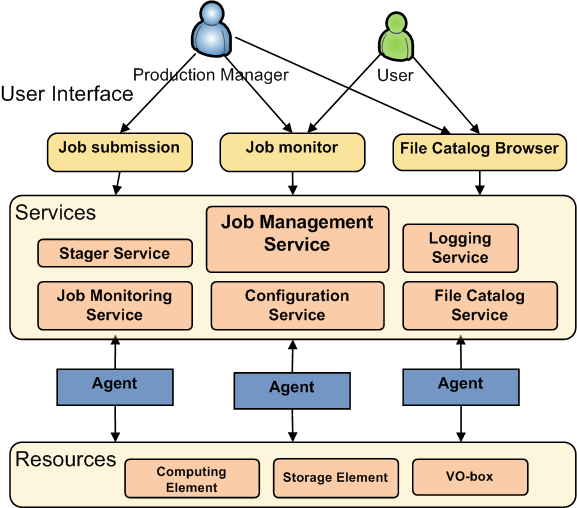
\includegraphics[height=5cm,keepaspectratio]{data/DIRAC_Architecture.png}
            \column{.4\linewidth}
                \begin{itemize}
                    \item User Interfaces
                    \item Services
                    \item Agents
                    \item Resources
                \end{itemize}
        \end{columns}
    \end{block}
\end{frame}

\begin{frame}
    \frametitle{Introduction to the Transfer System}
    \begin{itemize}
        \item In the transfer system, we have:
        \begin{itemize}
            \item {\tt Transfer Agent}.
            \item {\tt Transfer Request Service}.
            \item {\tt Dataset Service}.
        \end{itemize}
        \item {\tt Transfer Agent} is the scheduler to create the transfer 
              processes.
        \item {\tt Transfer Request Service} is to create and monitor the requests.
        \item {\tt Dataset Service} is to create a dataset. Because we don't have
              dataset support in DFC, we use this as a temporary solution.

    \end{itemize}
\end{frame}

\begin{frame}
    \frametitle{The Design of Transfer Agent}
    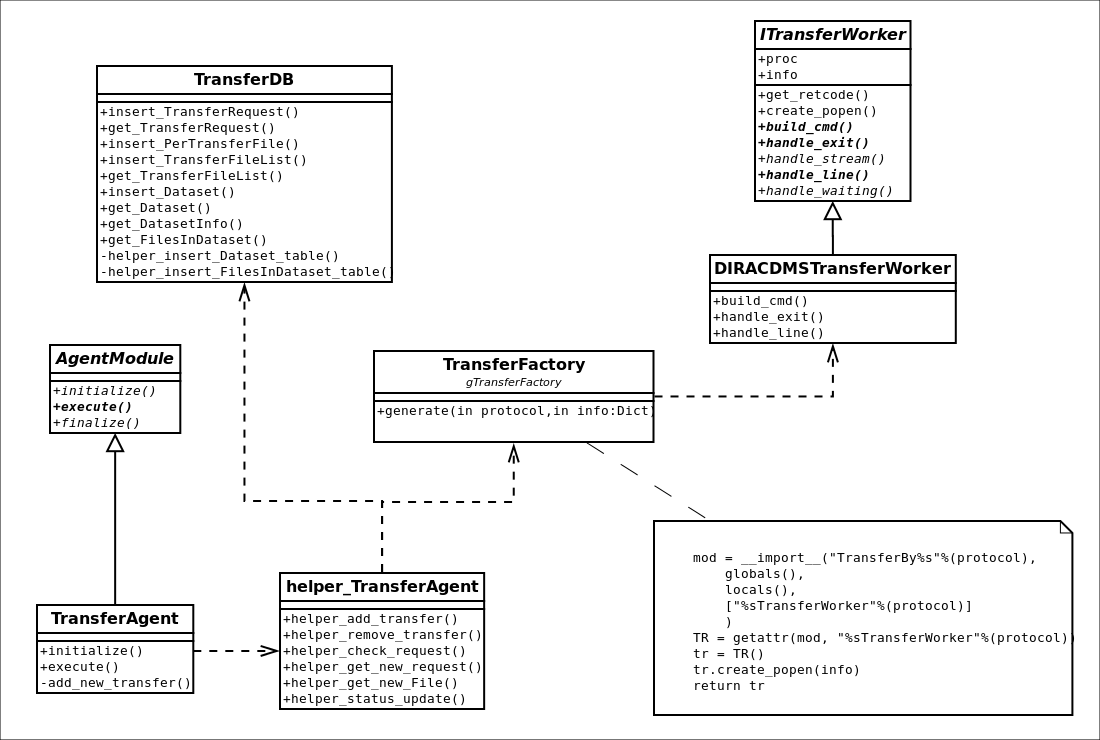
\includegraphics[height=8cm,keepaspectratio]{data/TransferAgent.png}
\end{frame}
